\documentclass{beamer}

\usepackage{graphicx}
\usepackage{tikz}
\usepackage{lmodern}
\usepackage{mathtools}
\usepackage{minted}

\usetheme{CambridgeUS}
\usecolortheme{beaver}
\setbeamercovered{transparent}
\usefonttheme{professionalfonts}
\setbeamertemplate{itemize items}[default]
\setbeamertemplate{caption}{\raggedright\insertcaption\par}
\begin{document}

\title[Compact finite differences on GPUs]
{A novel approach to evaluating 
compact finite differences 
and similar tridiagonal schemes on GPU-accelerated clusters}

\author[Ashwin Srinath]{
        Ashwin Srinath\\
        Department of Mechanical Engineering\\
        \today}
\date{}
\titlepage

\begin{frame}{Overview}
    \tableofcontents
\end{frame}

\section{Introduction}

\begin{frame}
\frametitle{Motivation}
\pause
\begin{itemize}[<+->]
    \item Computation established as the ``third way''
        to scientific truth
    \item Solving real problems:
        energy research,
        climate modeling,
        protein folding,
        quantum mechanics...
    \item Computational \emph{power} soon becomes
        the bottleneck for the size and scope of
        problems that can be solved
    \item Computational science and
        \emph{high-performance computing} have become
        synonymous
\end{itemize}
\end{frame}



\begin{frame}
\frametitle{Motivation}
\pause
\begin{itemize}[<+->]
    \item In \emph{direct numerical simulation},
        we aim to resolve all the spatial and temporal
        features of the flow.
    \item Use a fine computational grid
        and some high-accuracy numerical method to
        solve the flow equations on that grid.
    \item Among popular numerical methods
        are spectral methods, finite element methods,
        and finite difference methods
\end{itemize}
\end{frame}

\begin{frame}
\frametitle{Compact finite difference methods}
\pause
\begin{itemize}[<+->]
    \item Numerical estimation of derivatives
        is a keystone in scientific computation
    \item Simplest and most widely used approach
        is the \emph{finite difference} approximation
    \item In \emph{explicit} schemes,
        the derivative at some point $i$
        is expressed as a combination
        of function values at $i$ and other points
\end{itemize}
\end{frame}

\begin{frame}
\frametitle{Compact finite difference methods}
    \begin{figure}
    \includegraphics[width=150px]{img/discretize-function.eps}
    \caption{Uniformly sampling a function}
    \end{figure}
\end{frame}

\begin{frame}
\frametitle{Compact finite difference methods}
\begin{columns}[c]
     \begin{column}[T]{3cm}
        \begin{figure}
        \includegraphics[width=100px]{img/forward-difference.eps}
        \caption{Forward difference:
            derivative expressed in terms of function values
            at $i$, $i+1$, $i+2$, $\hdots$
        }
        \end{figure}
    \end{column}

     \begin{column}[T]{3cm}
        \begin{figure}
        \includegraphics[width=100px]{img/backward-difference.eps}
        \caption{Backward difference:
            derivative expressed in terms of function values
            at $\hdots$, $i-2$, $i-1$, $i$
        }
        \end{figure}
    \end{column}

    \begin{column}[T]{3cm}
        \begin{figure}
        \includegraphics[width=100px]{img/central-difference.eps}
        \caption{Central difference:
            derivative expressed in terms of function values
            at $\hdots$, $i-2$, $i-1$, $i$, $i+1$, $i+2$, $\hdots$
        }
        \end{figure}
    \end{column}
\end{columns}
\end{frame}

\begin{frame}
\frametitle{Compact finite difference methods}
\pause
\begin{itemize}[<+->]
    \item The schemes are \emph{explicit}
        because the derivative can be expressed
        at each point \emph{explicitly}
        as some combination of function values
    \item \emph{Compact} finite difference schemes
        express the derivative \emph{implicitly}:
    \item [] \begin{align*}
        \begin{split}
            f_i^{\prime} + \alpha(f^{\prime}_{i-1} + f^{\prime}_{i+1}) + \
            \beta(f^{\prime}_{i-2} + f^{\prime}_{i+2}) + \hdots \\
            = \\
            a\frac{f_{i+1} - f_{i-1}}{h} + \
            b\frac{f_{i+2} - f_{i-2}}{h} + \\
            c\frac{f_{i+3} - f_{i-3}}{h} + \
            \hdots
        \end{split}
        \label{eqn:general-compact}
        \end{align*}
\end{itemize}
\end{frame}

\begin{frame}
\frametitle{Graphics processing units}
\begin{columns}[c]
     \begin{column}[T]{5cm}
        Expectations
        \begin{figure}
        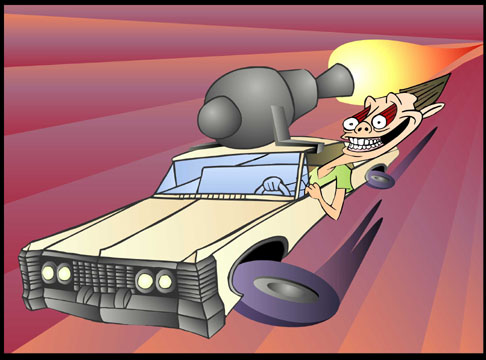
\includegraphics[width=150px]{img/expectations.jpg}
        \end{figure}
    \end{column}

    \begin{column}[T]{5cm}
        Reality
        \begin{figure}
        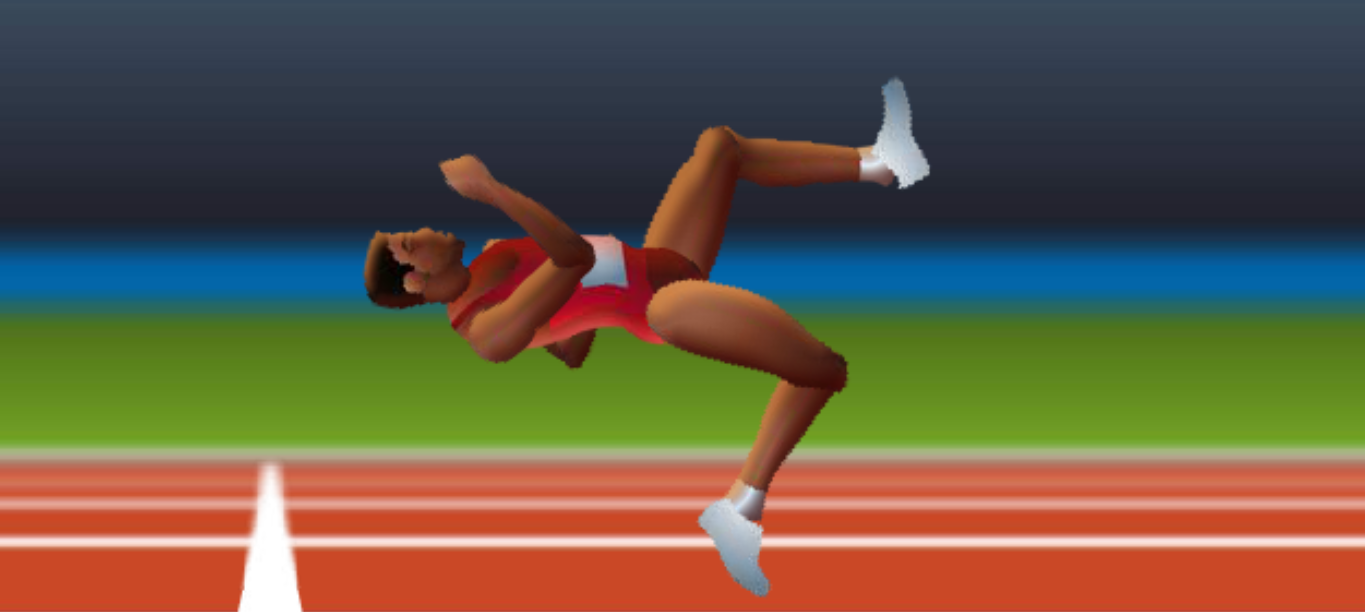
\includegraphics[width=150px]{img/reality.png}
        \end{figure}
    \end{column}
\end{columns}
\end{frame}

\begin{frame}[fragile]
  \begin{minted}{matlab}
      for i = 2:N-1
        dfdx(i) = (f(i+1) - f(i-1))/(2*dx)
      end
  \end{minted}
\end{frame}






\section{Proposed Tridiagonal Algorithm}
\section{Distributed Compact Finite Difference Evaluation}
\section{Results}

\end{document}
